\section{Estudio de Rendimiento}

Para el estudio de rendimiento de utilizo la cantidad de tiempo entre rutinas relevantes a cada prueba en milisegundos. Para obtener tiempos precisos en la \ac{GPU} se utilizó el software GPU PerfStudio y análisis de frame. Este software permite observar entre muchas otras cosas el tiempo total de cada llamada de dibujo o \emph{draw call} al API grafico OpenGL

\subsection{Prueba Base}
La prueba base de rendimiento comprende todos los pasos del algoritmo sin trazado de sombras o modificaciones sobre la escena estática. Para esta prueba se colocó la aplicación en actualización forzosa de tal manera que todos los pasos del algoritmo se realicen por frame. También se varían tres aspectos de la aplicación: resolución de pantalla, dimensión de la representación en vóxeles y factor de longitud de marcha del cono.

Para estas pruebas se utilizaron todas las escenas completas. La configuración del escenario consto de una luz direccional con mapeado de sombras y tres modelos precargados. Los modelos utilizados fueron Stanford Happy Buddha, Stanford Dragon y Stanford Bunny, seleccionados por su complejidad geométrica. Cada modelo tiene su propio material con un cono especular con apertura de 45, 27 y 9 grados respectivamente. La cámara en escena fue colocada de tal forma que todos los píxeles  visibles formen parte del trazado de conos. 

\begin{table}[h]
\centering
\begin{tabular}{llllllllll}
\rot{Escena}                    & \rot{Voxelización Estática} & \rot{Limpieza de Vóxeles Dinámicos} & \rot{Voxelización Dinámica} & \rot{Sombreado de Vóxeles} & \rot{Mipmapping Direccional} & \rot{Iluminación Global de Vóxeles} & \rot{Mipmapping Direccional} & \rot{Trazado de Conos con Vóxeles} & \rot{Tiempo Dinámico}    \\ \hline
\multicolumn{1}{|l|}{Sibenik}     & \multicolumn{1}{l|}{1.80}     & 0.58                                  & \multicolumn{1}{l|}{2.11}     & 0.95                         & \multicolumn{1}{l|}{1.39}      & 3.88                                  & \multicolumn{1}{l|}{1.38}      & \multicolumn{1}{l|}{7.31}            & \multicolumn{1}{l|}{17.60} \\
\multicolumn{1}{|l|}{Cornell Box} & \multicolumn{1}{l|}{0.51}     & 0.78                                  & \multicolumn{1}{l|}{1.30}     & 1.33                         & \multicolumn{1}{l|}{1.38}      & 8.41                                  & \multicolumn{1}{l|}{1.37}      & \multicolumn{1}{l|}{7.23}            & \multicolumn{1}{l|}{21.81} \\
\multicolumn{1}{|l|}{Conference}  & \multicolumn{1}{l|}{46.04}    & 0.56                                  & \multicolumn{1}{l|}{1.52}     & 0.86                         & \multicolumn{1}{l|}{1.38}      & 3.23                                  & \multicolumn{1}{l|}{1.37}      & \multicolumn{1}{l|}{7.50}            & \multicolumn{1}{l|}{16.42} \\
\multicolumn{1}{|l|}{Sponza}      & \multicolumn{1}{l|}{11.29}    & 0.60                                  & \multicolumn{1}{l|}{2.03}     & 1.13                         & \multicolumn{1}{l|}{1.37}      & 5.44                                  & \multicolumn{1}{l|}{1.38}      & \multicolumn{1}{l|}{7.01}            & \multicolumn{1}{l|}{18.97} \\ \hline
\end{tabular}
\captionsetup{justification=centering}
\caption{Rendimiento de todas las partes del algoritmo en distintas escenas utilizando volúmenes de resolución $256^3$, factor de longitud de marcha de $0.5$ y resolución de pantalla de $1280x720$. Todos los tiempos en milisegundos.}
\label{tab:performance_base}
\end{table}

\begin{table}[H]
\centering
\begin{tabular}{lllllllllll}
\rot{Resolucion de Volumenes}                 & \rot{Escena}                   & \rot{Voxelización Estática} & \rot{Limpieza de Vóxeles Dinámicos} & \rot{Voxelización Dinámica} & \rot{Sombreado de Vóxeles} & \rot{Mipmapping Direccional} & \rot{Iluminación Global de Vóxeles} & \rot{Mipmapping Direccional} & \rot{Trazado de Conos con Vóxeles} & \rot{Tiempo Dinámico}    \\ \hline
\multicolumn{1}{|l|}{\multirow{4}{*}{\rotv{$64^3$}}}  & \multicolumn{1}{l|}{Sibenik}     & \multicolumn{1}{l|}{3.00}     & 0.01                                  & \multicolumn{1}{l|}{9.17}     & 0.04                         & \multicolumn{1}{l|}{0.11}      & 0.12                                  & \multicolumn{1}{l|}{0.10}      & \multicolumn{1}{l|}{5.17}            & \multicolumn{1}{l|}{14.74} \\
\multicolumn{1}{|l|}{}                     & \multicolumn{1}{l|}{Cornell Box} & \multicolumn{1}{l|}{0.07}     & 0.02                                  & \multicolumn{1}{l|}{2.13}     & 0.06                         & \multicolumn{1}{l|}{0.11}      & 0.29                                  & \multicolumn{1}{l|}{0.11}      & \multicolumn{1}{l|}{4.79}            & \multicolumn{1}{l|}{7.51}  \\
\multicolumn{1}{|l|}{}                     & \multicolumn{1}{l|}{Conference}  & \multicolumn{1}{l|}{39.68}    & 0.01                                  & \multicolumn{1}{l|}{5.98}     & 0.03                         & \multicolumn{1}{l|}{0.11}      & 0.10                                  & \multicolumn{1}{l|}{0.11}      & \multicolumn{1}{l|}{5.38}            & \multicolumn{1}{l|}{11.72} \\
\multicolumn{1}{|l|}{}                     & \multicolumn{1}{l|}{Sponza}      & \multicolumn{1}{l|}{22.87}    & 0.01                                  & \multicolumn{1}{l|}{13.93}    & 0.05                         & \multicolumn{1}{l|}{0.17}      & 0.13                                  & \multicolumn{1}{l|}{0.17}      & \multicolumn{1}{l|}{5.49}            & \multicolumn{1}{l|}{19.97} \\ \hline
\multicolumn{1}{|l|}{\multirow{4}{*}{\rotv{$128^3$}}} & \multicolumn{1}{l|}{Sibenik}     & \multicolumn{1}{l|}{2.17}     & 0.08                                  & \multicolumn{1}{l|}{3.93}     & 0.17                         & \multicolumn{1}{l|}{0.26}      & 0.62                                  & \multicolumn{1}{l|}{0.26}      & \multicolumn{1}{l|}{2.17}            & \multicolumn{1}{l|}{3.93}  \\
\multicolumn{1}{|l|}{}                     & \multicolumn{1}{l|}{Cornell Box} & \multicolumn{1}{l|}{0.16}     & 0.10                                  & \multicolumn{1}{l|}{1.38}     & 0.28                         & \multicolumn{1}{l|}{0.26}      & 1.62                                  & \multicolumn{1}{l|}{0.26}      & \multicolumn{1}{l|}{5.75}            & \multicolumn{1}{l|}{1.38}  \\
\multicolumn{1}{|l|}{}                     & \multicolumn{1}{l|}{Conference}  & \multicolumn{1}{l|}{39.19}    & 0.07                                  & \multicolumn{1}{l|}{2.47}     & 0.15                         & \multicolumn{1}{l|}{0.26}      & 0.54                                  & \multicolumn{1}{l|}{0.26}      & \multicolumn{1}{l|}{6.42}           & \multicolumn{1}{l|}{2.47}  \\
\multicolumn{1}{|l|}{}                     & \multicolumn{1}{l|}{Sponza}      & \multicolumn{1}{l|}{15.15}    & 0.08                                  & \multicolumn{1}{l|}{4.00}     & 0.20                         & \multicolumn{1}{l|}{0.26}      & 0.82                                  & \multicolumn{1}{l|}{0.26}      & \multicolumn{1}{l|}{5.47}           & \multicolumn{1}{l|}{4.00}  \\ \hline
\multicolumn{1}{|l|}{\multirow{4}{*}{\rotv{$512^3$}}} & \multicolumn{1}{l|}{Sibenik}     & \multicolumn{1}{l|}{2.36}     & 4.51                                  & \multicolumn{1}{l|}{1.35}     & 6.06                         & \multicolumn{1}{l|}{10.92}     & 23.23                                 & \multicolumn{1}{l|}{10.91}     & \multicolumn{1}{l|}{8.57}            & \multicolumn{1}{l|}{65.55} \\
\multicolumn{1}{|l|}{}                     & \multicolumn{1}{l|}{Cornell Box} & \multicolumn{1}{l|}{6.18}     & 6.08                                  & \multicolumn{1}{l|}{1.80}     & 7.54                         & \multicolumn{1}{l|}{10.70}     & 41.14                                 & \multicolumn{1}{l|}{10.87}     & \multicolumn{1}{l|}{7.87}            & \multicolumn{1}{l|}{86.00} \\
\multicolumn{1}{|l|}{}                     & \multicolumn{1}{l|}{Conference}  & \multicolumn{1}{l|}{47.44}    & 4.46                                  & \multicolumn{1}{l|}{1.28}     & 5.63                         & \multicolumn{1}{l|}{11.57}     & 18.70                                 & \multicolumn{1}{l|}{11.35}     & \multicolumn{1}{l|}{8.56}            & \multicolumn{1}{l|}{61.56} \\
\multicolumn{1}{|l|}{}                     & \multicolumn{1}{l|}{Sponza}      & \multicolumn{1}{l|}{9.05}     & 4.55                                  & \multicolumn{1}{l|}{1.39}     & 6.87                         & \multicolumn{1}{l|}{11.16}     & 28.09                                 & \multicolumn{1}{l|}{10.79}     & \multicolumn{1}{l|}{7.64}            & \multicolumn{1}{l|}{70.49} \\ \hline
\end{tabular}
\captionsetup{justification=centering}
\caption{Rendimiento en contraste con la tabla \ref{tab:performance_base} considerando distintas resoluciones para la representación en vóxeles, todos los pasos del algoritmo se ven afectados por este parámetro.}
\label{tab:performance_depth}
\end{table}
\begin{table}[H]
\centering
\begin{tabular}{|l|l|l|}
\hline
Resolución Pantalla  & 1920x1080                    & 1280x720                     \\ \hline
Escena      & Trazado de Conos con Vóxeles & Trazado de Conos con Vóxeles \\ \hline
Sibenik     & 14.30                        & 7.31                         \\
Cornell Box & 15.17                        & 7.23                         \\
Conference  & 16.27                        & 7.50                         \\
Sponza      & 16.69                        & 7.01                         \\ \hline
\end{tabular}
\captionsetup{justification=centering}
\caption{Rendimiento con una mayor resolución de pantalla. Esto solo afecta el trazado de conos con vóxeles.}
\label{tab:performance_display}
\end{table}
\begin{table}[H]
\centering
\begin{tabular}{|l|l|l|l|l|}
\hline
Longitud de Marcha & 0.1         & 0.25        & 0.5       & 2.5       \\ \hline
Escena             & \multicolumn{4}{l|}{Trazado de Conos con Vóxeles} \\ \hline
Sibenik            & 29.55       & 12.73       & 7.31      & 2.67      \\
Cornell Box        & 26.80       & 11.57       & 7.23      & 2.68      \\
Conference         & 29.73       & 12.93       & 7.50      & 2.85      \\
Sponza             & 29.81       & 12.92       & 7.01      & 2.81      \\ \hline\end{tabular}
\captionsetup{justification=centering}
\caption{Rendimiento con distintas configuraciones de la longitud de marcha del cono. Esto solo afecta el trazado de conos con vóxeles.}
\label{tab:performance_step}
\end{table}

Considerando como tiempos interactivos todo resultado por debajo de $33.3 ms$ o aproximadamente 30 cuadros por segundo. Nuestra implementación logra colocarse por debajo de este tiempo en todos los casos excepto los casos que comprenden resoluciones de volúmenes mayores a $256^3$.

\subsubsection{Densidad Geométrica y Velocidad de Voxelización.}
La cantidad de triángulos dentro del espacio que representa un vóxel afecta la velocidad de voxelización. Esto se debe a que este proceso requiere sincronización entre distintos hilos por fragmento. A mayor cantidad de triángulos en este espacio mayor es la cantidad de fragmentos generados por el proceso de rasterización. Cada uno de estos hilos debe esperar a escribir en la misma posición del volumen para garantizar atomicidad.

En la imagen \ref{fig:voxelization_times} se puede observar esta condición, especialmente en la escena Conference. Esta es una escena pequeña en escala, sin embargo de todas las escenas completas es la que posee mayor cantidad de triángulos como se puede observar en la tabla \ref{tab:scenes_attributes}. También es notable como disminuye el tiempo de voxelización para algunas escenas al aumentar la resolución del volumen y como aumenta al utilizar menores resoluciones, especialmente el salto entre $128^3$ a $64^3$.

\begin{figure}[H]
	\centering
	\begin{subfigure}{.49\textwidth}
		\centering
		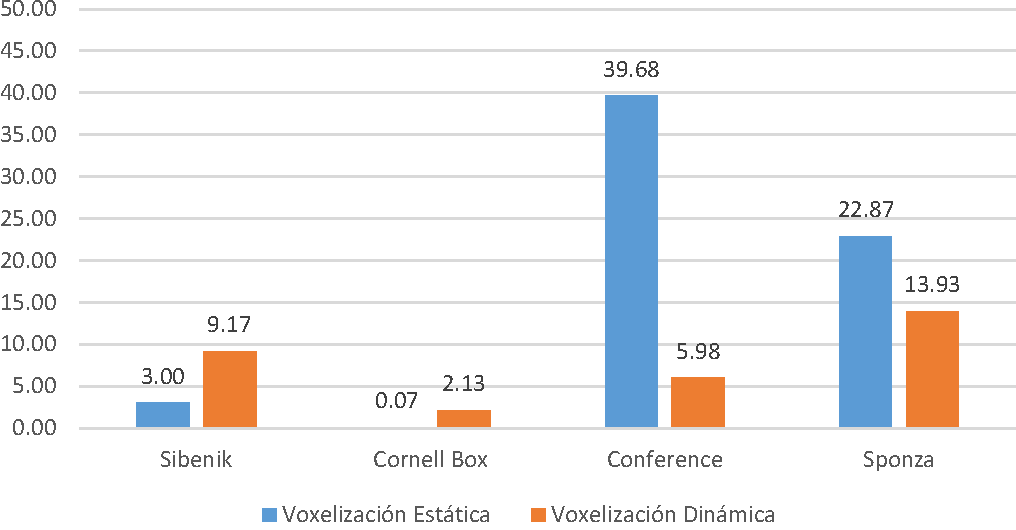
\includegraphics[width=\linewidth]{media/voxelzation_64_cropped.pdf}
		\caption*{Resolución de volúmenes: $64^3$}
	\end{subfigure}
	\begin{subfigure}{.49\textwidth}
		\centering
		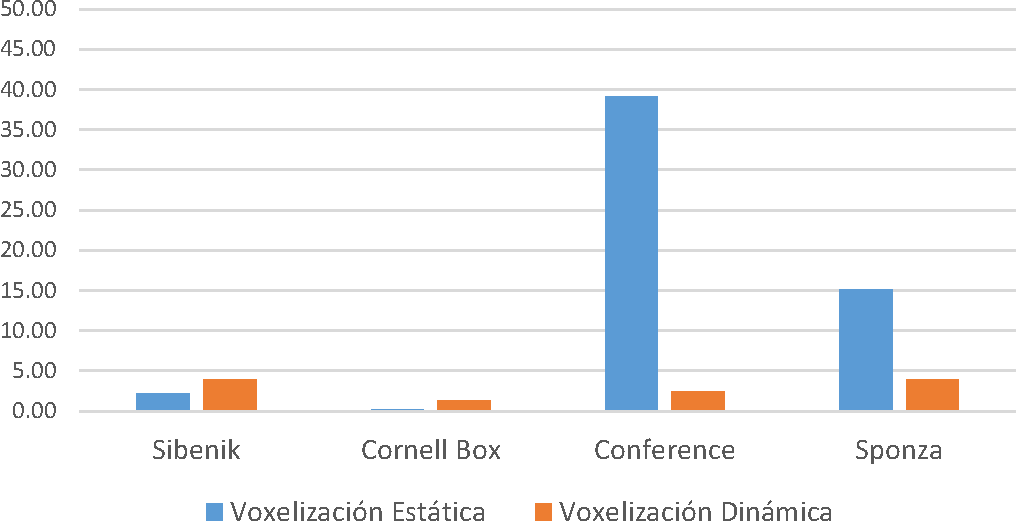
\includegraphics[width=\linewidth]{media/voxelzation_128_cropped.pdf}	
		\caption*{Resolución de volúmenes: $128^3$}
	\end{subfigure}
	\par\bigskip
	\begin{subfigure}{.49\textwidth}
		\centering
		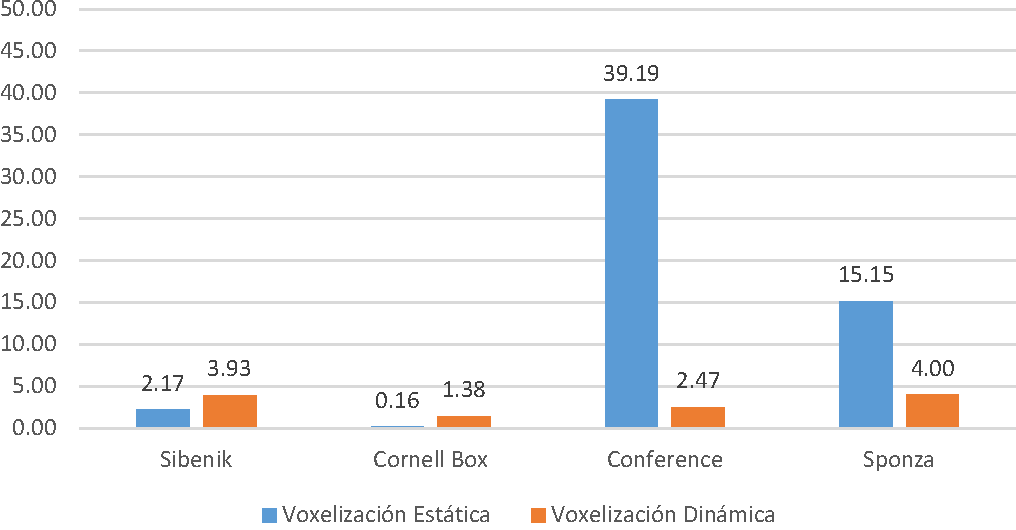
\includegraphics[width=\linewidth]{media/voxelzation_256_cropped.pdf}
		\caption*{Resolución de volúmenes: $256^3$}
	\end{subfigure}
	\begin{subfigure}{.49\textwidth}
		\centering
		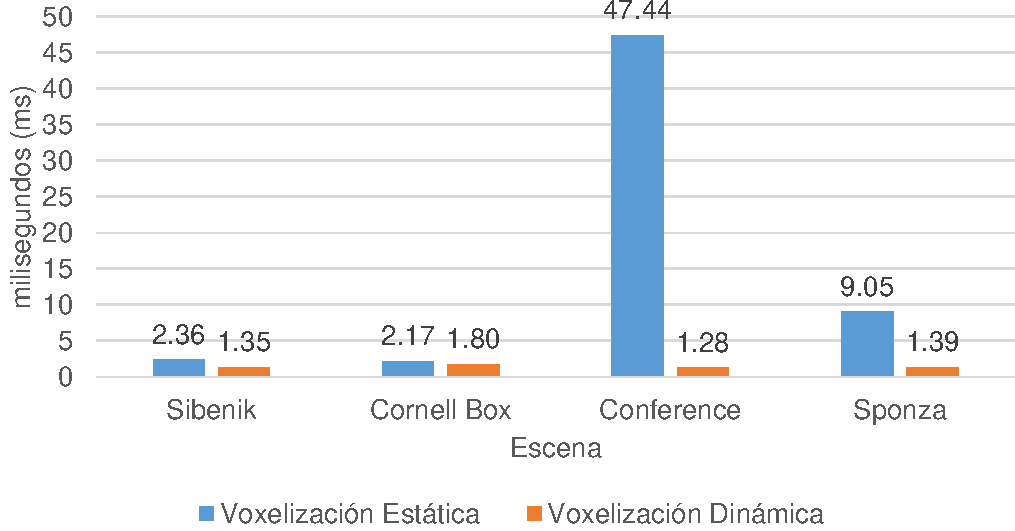
\includegraphics[width=\linewidth]{media/voxelzation_512_cropped.pdf}	
		\caption*{Resolución de volúmenes: $512^3$}
	\end{subfigure}
	\caption{Tiempos de voxelización dinámica y estática de escenas completas con distintas resoluciones para la representación en vóxeles. Tabla \ref{tab:performance_depth}}
	\label{fig:voxelization_times}
\end{figure}

\subsubsection{Vacuidad y Velocidad de Trazado para la Iluminación Global de Vóxeles.}
\label{subsubsec:emptyness}

En escenas donde existen muchos espacios vacíos el trazado de rayos suele tardar un poco más que en escenas densas de objetos. Esto se debe a que mientras la representación en vóxeles sea vacía en la posición que describe la apertura, dirección y punto de origen del cono, este cono debe seguir expandiéndose. A consecuencia mientras más espacios vacíos la representación en vóxeles tenga, más distancia tiene que recorrer cada cono aumentando la cantidad de operaciones de lectura sobre la representación en vóxeles.

Este problema se puede observar en la figura \ref{fig:gi_voxel_time} para las escenas Sponza y Cornell Box. La escena Cornell Box es en gran parte vacua con solo dos cuboides internos. La escena Sponza es densa en su interior por tanto la falta de objetos no es el principal problema. El problema de la Sponza reside en que la escena es larga y alta pero no ancha. Durante la voxelización cada triángulo se proyecta de forma ortogonal sobre cada eje para maximizar la voxelización, este frustum de proyección es cuadrado. Para las dimensiones de esta escena siempre quedara una cantidad considerable de vóxeles vacíos fuera de la geometría principal de la escena. 

% Una forma de evitar estos problemas en escenas como Sponza es comprobar que la posición de trazado actual está fuera de los límites de la escena, sin embargo esto puede ocasionar problemas visuales dependiendo de la apertura del cono en ese punto, para limitar correctamente el punto de trazado con respecto a los límites de la escena es necesario calcular la intersección del cono contra el volumen delimitante.

\begin{figure}[h]
	\centering
	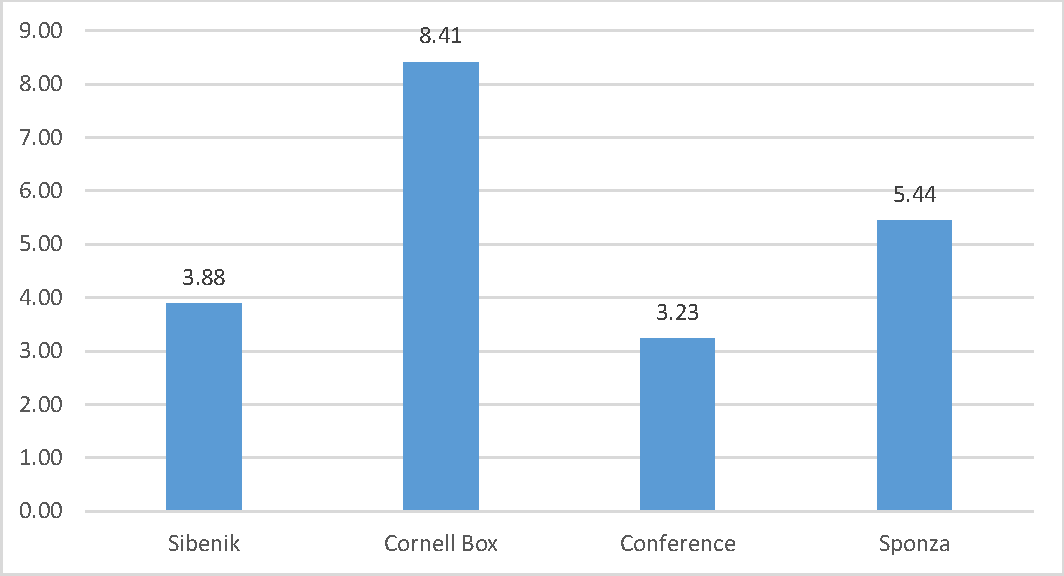
\includegraphics[width=0.95\linewidth]{media/voxel_gi_time_cropped.pdf}
	\caption{Tiempos de cálculo de iluminación global sobre la representación en vóxeles para todas las escenas completas.}
	\label{fig:gi_voxel_time}
\end{figure}

\subsection{Trazado de Sombras y Volumen de Visibilidad}

La aplicación provee sombras suaves para luces direccionales, puntuales y focales utilizando trazado de conos. Si no se sombrea la representación en vóxeles la imagen resultante es incorrecta a pesar de definir los contornos de sombreado. La razón es que el trazado de conos para la iluminación indirecta consideraría estos vóxeles como iluminados en vez de ocluidos por sombras. Nuestra implementación provee un método de inclusión de sombras suaves durante el sombreado de vóxeles. En esta sección se examina el rendimiento de las distintas opciones para el trazado de sombras que provee nuestra implementación excepto mapeado de sombras (sección \ref{subsec:shadowmapping}) disponible solo para luces direccionales.

Para estas pruebas se utilizaron todas las escenas completas. La configuración del escenario consto de solo una luz puntual con trazado de sombras habilitado. La cámara en escena fue colocada de tal forma que todos los píxeles visibles formen parte del trazado de conos. 

Con respecto a la configuración de la aplicación, se activó el modo de actualización forzosa para simular luces en constante movimiento y se desactivo la iluminación global de vóxeles. La resolución de la representación en vóxeles utilizada fue de $256^3$ y el factor de longitud de marcha del cono fue $0.5$.

Este estudió considera las distintas opciones en la aplicación relevantes al trazado de sombras. Estas opciones comprenden: trazado de sombras durante el sombreado de vóxeles, trazado de sombras con trazado de conos y vóxeles o muestreo del volumen de visibilidad.

\begin{table}[h]
\centering
\begin{tabular}{lll}
                                  &                                           &                                                                \\ \hline
\multicolumn{1}{|l|}{Escena}      & \multicolumn{1}{l|}{Sombreado de Voxeles} & \multicolumn{1}{l|}{Sombreado y Trazado de Sombras} \\ \hline
\multicolumn{1}{|l|}{Sibenik}     & \multicolumn{1}{l|}{0.95}                 & \multicolumn{1}{l|}{4.57}                                      \\
\multicolumn{1}{|l|}{Cornell Box} & \multicolumn{1}{l|}{1.33}                 & \multicolumn{1}{l|}{20.32}                                     \\
\multicolumn{1}{|l|}{Conference}  & \multicolumn{1}{l|}{0.86}                 & \multicolumn{1}{l|}{4.77}                                      \\
\multicolumn{1}{|l|}{Sponza}      & \multicolumn{1}{l|}{1.13}                 & \multicolumn{1}{l|}{3.31}                                      \\ \hline
\end{tabular}
\caption{Tiempos de sombreado de vóxeles con y sin trazado de sombras sobre el volumen.}
\label{tab:voxelshading_shadowing}
\end{table}

\begin{figure}[h]
	\centering
	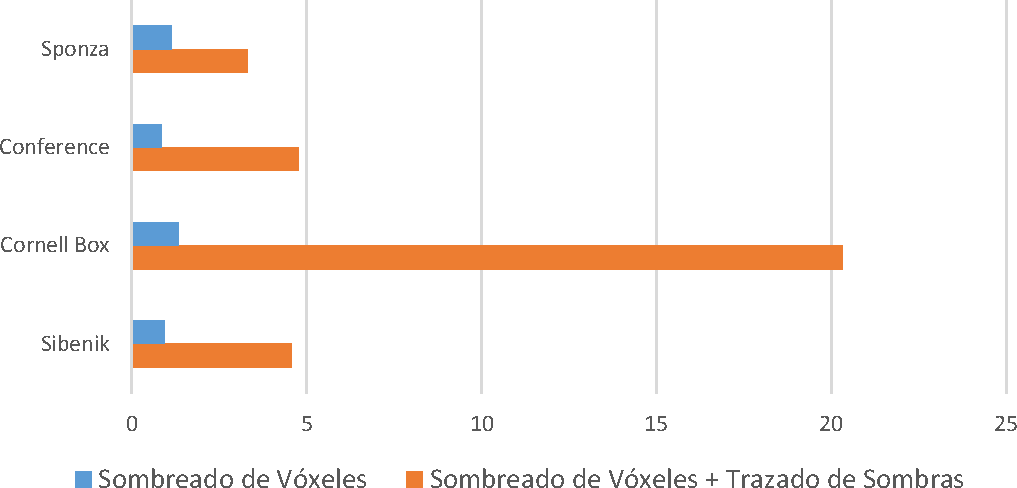
\includegraphics[width=0.95\linewidth]{media/voxelshading_shadow_cropped.pdf}
	\caption{Grafica para el tiempo agregado al sombreado de vóxeles con trazado de sombras. Tabla \ref{tab:voxelshading_shadowing}.}
	\label{fig:voxelshading_shadowing}
\end{figure}

En la imagen \ref{fig:voxelshading_shadowing} se puede observar un incremento del tiempo de cómputo invertido durante el sombreado de vóxeles al incluir sombras trazadas sobre el volumen. En la escena Cornell Box este incremento es mucho mayor al de las demás escenas. La razón es que esta escena es en gran parte vacía, por lo tanto la mayoría de los rayos trazados tienen que recorrer un largo camino antes de culminar. Sin embargo, la escena Sponza a pesar de tener los mismos problemas de vacuidad ya explicados en la sección \ref{subsubsec:emptyness} tiene un tiempo agregado similar a las demás escenas sin estos problemas. Esto se debe principalmente a que la fuente de luz puntual se encuentra en el interior de la escena. La posición de la fuente de luz a trazar en la escena afecta directamente el rendimiento, ya que esta determina en promedio que tan rápido la mayoría de los rayos terminan su recorrido.

\begin{table}[H]
\centering
\begin{tabular}{llll}
                                  &                                       &                                             &                                         \\ \hline
\multicolumn{1}{|l|}{Escena}      & \multicolumn{1}{l|}{Trazado de Conos} & \multicolumn{1}{l|}{Volumen de Visibilidad} & \multicolumn{1}{l|}{Conos para Sombras} \\ \hline
\multicolumn{1}{|l|}{Sibenik}     & \multicolumn{1}{l|}{7.31}             & \multicolumn{1}{l|}{6.03}                   & \multicolumn{1}{l|}{8.58}               \\
\multicolumn{1}{|l|}{Cornell Box} & \multicolumn{1}{l|}{7.23}             & \multicolumn{1}{l|}{6.50}                   & \multicolumn{1}{l|}{10.31}              \\
\multicolumn{1}{|l|}{Conference}  & \multicolumn{1}{l|}{7.50}             & \multicolumn{1}{l|}{5.65}                   & \multicolumn{1}{l|}{5.65}               \\
\multicolumn{1}{|l|}{Sponza}      & \multicolumn{1}{l|}{7.01}             & \multicolumn{1}{l|}{6.28}                   & \multicolumn{1}{l|}{8.30}               \\ \hline
\end{tabular}
\caption{Tiempo agregado al paso de trazado de conos con vóxeles al incluir trazado de sombras con conos.}
\label{tab:shadowcone5}
\end{table}

\begin{figure}[H]
	\centering
	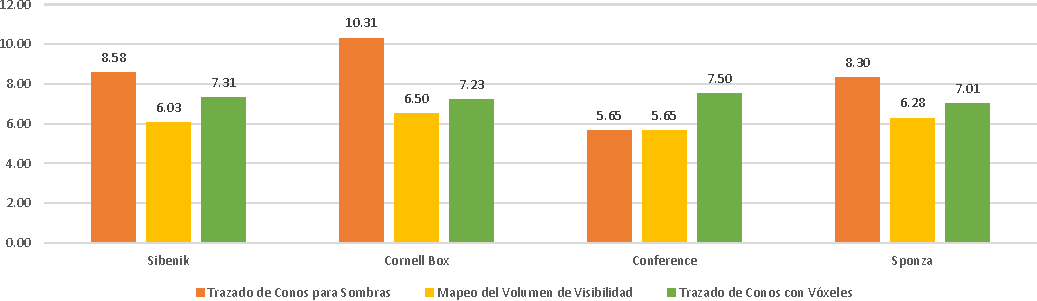
\includegraphics[width=0.95\linewidth]{media/shadowtrace_time_cropped.pdf}
	\caption{Grafica para el tiempo agregado al trazado de conos con vóxeles utilizando conos para sombras suaves o mapeo del volumen de visibilidad. Tabla \ref{tab:shadowcone5}.}
	\label{fig:voxeltrace_shadowing}
\end{figure}

El mapeo del volumen de visibilidad ofrece mayor rendimiento a cambio de menor calidad de sombras. El trazado de conos con vóxeles incluye el tiempo invertido en mapeo de sombras en la prueba base \ref{tab:performance_base}. En contraste el mapeo del volumen de visibilidad es mucho más rápido ya que este solo es una instrucción de lectura más una simple operación aritmética para convertir la posición en espacio de mundo a una coordenada en espacio de textura. En algunos casos el trazado de conos para sombras puede incluso ser más rápido que la técnica de mapeo de sombras. Esto se observa en la escena Conference, la razón es que esta es una escena pequeña en escala y densa en geometría, los conos trazados suelen terminar rápidamente.

\subsection{Apertura del Cono Especular y Cono de Sombras}

La apertura de los conos a trazar afecta directamente el rendimiento del trazado de conos con vóxeles. Mientras más fino es este cono más lenta es su expansión a través del espacio en escena ya que el incremento de la longitud de marchado es mucho más lenta. También mientras más fino es este cono mayor tiempo se invierte en los niveles más altos de detalle en la representación de vóxeles, en la tabla \ref{tab:performance_depth} se puede observar que a mayor resolución del volumen mayor es el tiempo de trazado.

El objetivo de estas pruebas es demostrar la diferencia en rendimiento según distintas configuraciones de apertura del cono especular y el cono utilizado para el trazado de sombras suaves.

Para ambas pruebas se utilizó solo la escena completa Cornell Box. Para la prueba del cono de sombras se colocó dentro de la escena una luz puntual con trazado de sombras habilitado. Para la prueba del cono especular se colocó dentro la escena una esfera con un material especular y una luz puntual con trazado de sombras inhabilitado. Para ambas pruebas la resolución de la representación en vóxeles y la longitud de marcha del cono es de $256^3$ y $0.5$ respectivamente. El ángulo de apertura para ambas pruebas es 1, 5, 20, y 45 grados.

\begin{figure}[H]
	\centering
	\begin{subfigure}{.7\textwidth}
		\centering
		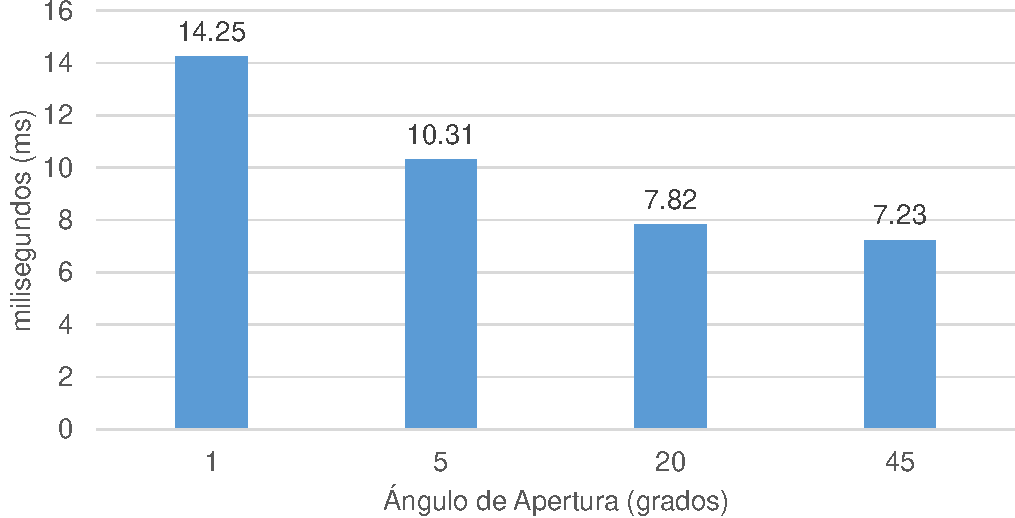
\includegraphics[width=\linewidth]{media/shadowcone_aperture_cropped.pdf}
		\caption{Tiempo de trazado de conos con vóxeles con distintas aperturas del cono para el trazado de sombras suaves.}
		\label{fig:shadowcone_aperture}
	\end{subfigure}
	\par\bigskip
	\begin{subfigure}{.7\textwidth}
		\centering
		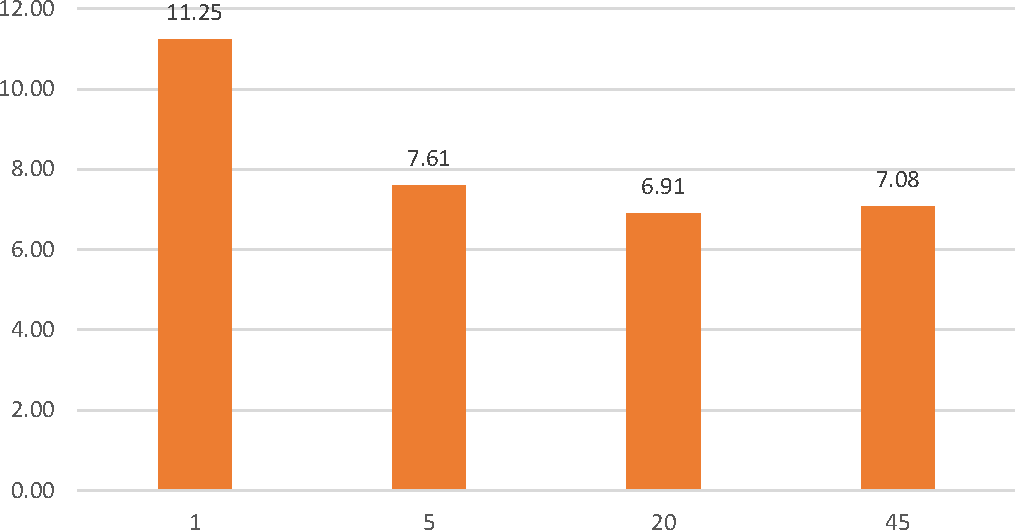
\includegraphics[width=\linewidth]{media/specularcone_aperture_cropped.pdf}
		\caption{Tiempo de trazado de conos con vóxeles con distintas aperturas del cono especular.}
		\label{fig:specularcone_aperture}
	\end{subfigure}
\end{figure}
